\documentclass[letterpaper,10pt]{article}
\usepackage[utf8x]{inputenc}
\usepackage{graphicx,color}

% Construct the basic page sizes
\oddsidemargin  0.0in
\evensidemargin 0.0in
\textwidth      6.5in
\headheight     0.25in
\topmargin      0.0in
\textheight=8.5in


%opening
\title{Adding Physical Models to GMAT}
\author{Darrel J. Conway\\Thinking Systems, Inc.}

\begin{document}

\maketitle

\begin{abstract}
This document describes the steps needed to add a new PhysicalModel to GMAT. 
It includes information about populating the orbital A-matrix and the orbital
State Transition Matrix.  It does not include information about adding new
states (e.g. quaternions for attitude dynamics) to the propagation state vector.
\end{abstract}

\section{Overview}

GMAT's Propagation Subsystem consists of a collection of classes that work
together to evolve elements of a mission over time.  The base classes for this
subsystem are shown in Figure~\ref{fig:BasePropClasses}.  The Propagation
subsystem is driven from one of several commands designed to use a propagation
configuration.  Commands that work with the propagation subsystem are all
derived from the PropagationEnabledCommand base class.  Those classes all use
the interfaces in the PropSetup class and in the Propagator and ODEModel
classes to function, so they are not described here.  Instead, this document
describes the interfaces that are needed in the classes derived
from PhysicalModel that the ODEModel depends on to function correctly. This
overview is intended to provide background information about the interactions
between classes that may help in building new physical models.

\begin{figure}[htb]
\begin{centering}
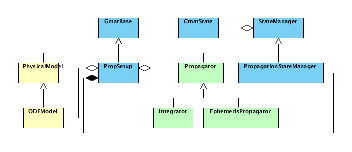
\includegraphics[scale=2.5]{./AddPhysicalModelImages/CorePropSubsystem.eps}
\caption{Base Classes of the Propagation Subsystem}
\label{fig:BasePropClasses}
\end{centering}
\end{figure}

The classes shown in Figure~\ref{fig:BasePropClasses} play the following roles:

\begin{description}
\item \textbf{GmatState}

This class models a collection of real number data with an associated epoch. 
It contains a vector of real data, an epoch, a mapping between data elements
and other associated elements in the vector, IDs for the data elements, and
strings describing each element. GMAT's propagation subsystem constructs and
uses a GmatState object as the core data structure that evolves over time. 
This object, called the propagation state vector, is designed to be flexible,
and to grow or shrink depending on the needs of the mission being modeled. 

\item \textbf{PropSetup}

The PropSetup class is a container class that collect a
PropagationStateManager, Propagator, and optionally an ODEModel into a single
object for use by a PropagationEnabledCommand.  The PropSetup objects present
the publicly visible elements of an instance of a configured propagation
configuration. For example, changes to the ``Propagator'' in the GMAT GUI
actually make changes to a PropSetup object.

\item \textbf{Propagator}

Propagator is the base class for all of GMAT's evolution operators.  The
Propagator class defines the interface for advancing a propagation state vector
from some initial time $t_i$ to a final time $t_f$.  Derived classes implement
the specific evolution operator, and hence determine if an ODEModel is required.

\item \textbf{Integrator}

Numerical integration is performed in GMAT by a class derived from the
Integrator base class.  Integrators require an ODEModel to function correctly. 
The Integrator class is further subclassed into a RungeKutta class, a
PredictorCorrector class, and other classes based on the numerical integration
algorithm needed.

\item\textbf{EphemerisPropagator}

GMAT is designed with the ability to evolve a state vector using analytic
methods, either from a set of analytic equations or by interpolating from a data
file.  The latter case works from interfaces defined in the EphemerisPropagator
class. The first case of an ephemeris propagator in GMAT is the SPK
propagator.

\item \textbf{PhysicalModel}

PhysicalModel is the base class for objects that provide differential equation
data to the Integrator classes.  The PhysicalModel class is subclassed to
implement a specific set of differential equations that are then called by the
numerical integrators.  There is one special PhysicalModel class, the ODEModel,
which is used to accumulate derivative data for the Integrators. 
Figure~\ref{fig:PhysicalModels} shows the PhysicalModels in GMAT at this
writing.

\item \textbf{ODEModel}

The ODEModel class implements the accumulation of derivative information
required when performing numerical integration.  ODEModel objects are
containers for collections of PhysicalModels that together define the physics
used to evolve a state vector. They apply superposition to the data generated
by each member PhysicalModel, add the results together, and report the results
to the numerical integrators.  They can also optionally generate the A-matrix
and the derivative of the state transition matrix for use in other calculations.

\item\textbf{PropagationStateManager}

The PropagationStateManager is a helper class that manages the state vector
that is propagated in the propagation subsystem.  The PropagationStateManager
tracks the state members element by element, associations between the elements,
and constructs the state vector for use by Propagator and ODEModel objects.

\end{description}

The classes described, and classes derived from them, above comprise the
propagation subsystem.  The subsystem can be extended on either the Propagator
side of the class hierarchy or on the PhysicalModel side.  New integrators and
propagators are added to the system to implement new techniques for evolving
a propagation state vector.  New forces or other derivative models are added by
adding subclasses of the PhysicalModel class.  The remainder of this document
describes the latter operation: extending the derivative models by implementing
new PhysicalModel classes.

\begin{figure}[htb]
\begin{centering}
\includegraphics[scale=2.5]{./AddPhysicalModelImages/PhysicalModels.eps}
\caption{Physical Model Classes}
\label{fig:PhysicalModels}
\end{centering}
\end{figure}

Figure~\ref{fig:PhysicalModels} shows the core PhysicalModel classes in GMAT
that provide data for specific portions of the physics modeled by Integrators. 
The next section describes the interfaces that are required in order for a
PhysicalModel object to interact with an ODEModel object.  Following that
section you will find specific instructions for adding the model to GMAT's
factory subsystem, and then instructions for adding ancillary objects that are
used by a PhysicalModel, using an atmosphere model for the DragForce as an
example.

\section{Creating the Model}

The basic approach to adding a force or other derivative model to GMAT starts
with designing and coding the class implementing the new model.  The steps
involved are basically these:

\begin{itemize}
\item Create a C++ class for the new model. 
\item Derive the new class from PhysicalModel (or a class derived from
PhysicalModel).
\item Implement at a minimum the following methods:
\begin{itemize}
\item The usual four methods: \textbf{Constructor}, \textbf{Destructor},
\textbf{Copy Constructor} and \textbf{Assignment operator} (aka operator=).  All
GMAT classes that are derived from GmatBase need these methods to work correctly
with GMAT's Configuration/Sandbox cloning design.
\item\textbf{Clone}:  GmatBase defines this method as an abstract method to be
implemented in all leaf classes.  You'll need to implement it to call your
class's copy constructor. 
\item \textbf{Initialize}:  Use this method to perform the final setup of your
model prior to use by an integrator.  This method is not strictly required, but
is nearly always needed so that the model can adapt to changing state vector
sizes and other dynamic propertied that may affect the derivative calculations.
\item \textbf{SupportsDerivative}:  This method identifies the supported
derivative types for the model.  By default, the Gmat::CARTESIAN\_STATE type is
supported.  Other options include MASS\_FLOW, ORBIT\_STATE\_TRANSITION\_MATRIX,
and the ORBIT\_A\_MATRIX (all defined in the Gmat namespace).
\item \textbf{SetStart}:  The ODEModel uses this method to set the index for the
start and size of supported derivative types. 
\item \textbf{IsUserForce}:  (Optional)  This method identifies PhysicalModels
incorporated though the plugin interface, or through other means outside of the
standard forces managed in GMAT's Interpreter code.
\item \textbf{GetDerivatives}:  The GetDerivatives method is the method accessed
by an ODEModel to build the total state derivative.
\end{itemize}
\end{itemize}

\noindent The following paragraphs provide additional information about the last
four of these methods, and include some stripped down sample code for each.

\subsection{The SupportsDerivative Method}

The SupportsDerivative method has the signature

\begin{quote}
\begin{verbatim}
virtual bool SupportsDerivative(Gmat::StateElementId id);
\end{verbatim}
\end{quote}

\noindent The purpose of this method is to identify support for specific
derivative components inside of a PhysicalModel.  It returns true if the input
derivative type is supported, and false if not.  Thus the code for the
FiniteThrust PhysicalModel, which currently supports derivatives of the
Cartesian state and mass depletion but no other derivative data, looks like
this:

\begin{quote}
\begin{verbatim}
bool FiniteThrust::SupportsDerivative(Gmat::StateElementId id)
{
   if (id == Gmat::CARTESIAN_STATE)
      return true;
   
   if (id == Gmat::MASS_FLOW)
      return true;
   
   return PhysicalModel::SupportsDerivative(id);
}
\end{verbatim}
\end{quote}

\noindent If support is added for the A-matrix, another if test will be added
to this method.  Otherwise, the ODEModel will simply ignore this model when
accumulating A-matrix data for an Integrator.

\subsection{The SetStart Method}

The SetStart method sets the index values for specific derivative data into the
propagation state vector.  It provides data used by the GetDerivatives method
to fill in the data needed for the derivative calculations.  The method has the
signature

\begin{quote}
\begin{verbatim}
virtual bool SetStart(Gmat::StateElementId id, Integer index, 
                         Integer quantity);
\end{verbatim}
\end{quote}

\noindent One example of this method is that found in the
SolarRadiationPressure model:

\begin{quote}
\begin{verbatim}
bool SolarRadiationPressure::SetStart(Gmat::StateElementId id, Integer index, 
                      Integer quantity)
{
   bool retval = false;
   
   switch (id)
   {
      case Gmat::CARTESIAN_STATE:
         satCount = quantity;           // Deprecated!
         cartesianCount = quantity;
         cartesianStart = index;
         fillCartesian = true;
         retval = true;
         break;
         
      case Gmat::ORBIT_STATE_TRANSITION_MATRIX:
         stmCount = quantity;
         stmStart = index;
         fillSTM = true;
         retval = true;
         break;
         
      case Gmat::ORBIT_A_MATRIX:
         aMatrixCount = quantity;
         aMatrixStart = index;
         fillAMatrix = true;
         retval = true;
         break;

      default:
         break;
   }
   
   return retval;
}
\end{verbatim}
\end{quote}

\noindent The propagation state vector is arranged by data type; all of the
Cartesian state data is grouped together in one section, mass flow data in
another, and so forth.  The PhysicalModel class includes data structures to
track the size and location of each known type in internal protected variables
named \textit{typename}Count, \textit{typename}Start, and fill\textit{Typename},
where \textit{typename} identifies the type of state element in the vector. 
These data elements are populated in the SetStart method; this method provides
the basic starting points for populating the derivative data in the propagation
state vector.

\subsection{The IsUserForce Method}

Scripting for the ODEModel in GMAT is currently coded so that the core forces
are managed in the Interpreter code on a case-by-case basis.  The addition of
new forces allows for new capabilities in GMAT, but these new cases have to
handled differently from the scripting side of the system.  Users identify
these new, not yet fully interpreted cases by setting the IsUserForce method to
return true.  The signature for this method is

\begin{quote}
\begin{verbatim}
virtual bool IsUserForce();
\end{verbatim}
\end{quote}

\noindent When the implementation returns true -- as in the solar sail code from
the Plugin repository at SourceForge:

\begin{quote}
\begin{verbatim}
bool SolarSailForce::IsUserForce()
{
   return true;
}
\end{verbatim}
\end{quote}

\noindent then the Interpreter identifies the new derivative model from
scripting calling out the force from a list of user defined forces:

\begin{quote}
\begin{verbatim}
Create ForceModel Prop_ForceModel;
...
GMAT Prop_ForceModel.UserDefined = {SailForce};
\end{verbatim}
\end{quote}

\subsection{The GetDerivatives Method}

The heart of GMAT's PhysicalModel system is the GetDerivatives method.  This
method is called repeatedly during propagation -- as often as sixteen times per
propagation step with the current suite of numerical integrators -- so the
method must be coded with efficiency in mind in order to enhance GMAT's
performance.  The method has the signature

\begin{quote}
\begin{verbatim}
virtual bool GetDerivatives(Real * state, Real dt = 0.0, Integer order = 1, 
         const Integer id = -1);
\end{verbatim}
\end{quote}

\noindent where \texttt{state} is a vector of state data managed in the
propagator, \texttt{dt} is a time offset from a base epoch, measured in
seconds, \texttt{order} determines if the order of the derivative is first or
second based on the needs of the Integrator, and \texttt{id} is a flag for the
specific type of derivative requested.  The last parameter, \texttt{id}, is not
used in the current GMAT code. 

When the GetDerivatives model is called on a Physical Model, the algorithm for
the PhysicalModel takes the input state and fills in derivative information in
an internal data structure named \texttt{derivs}, defined in the PhysicalModel
base class.  An overview of this process can be seen in a stripped down version
of the PointMassForce code:

\begin{quote}
\begin{verbatim}
bool PointMassForce::GetDerivatives(Real * state, Real dt, Integer order, 
      const Integer id)
{
   Integer i6, a6;

   if (fillCartesian || fillSTM || fillAMatrix)
   {
      Real radius, r3, mu_r, rbb3, mu_rbb, a_indirect[3];

      // Set up data that applies throughout the calculations
      epoch = theState->GetEpoch();
      now = epoch + dt/GmatTimeConstants::SECS_PER_DAY;
...
      
      if (fillCartesian)
      {
         for (Integer i = 0; i < satCount; i++) 
         {
            i6 = cartesianStart + i * 6;

            // Calculate some data used in each element
            ...

            // Then fill in the Cartesian state derivatives; 
            // left intact for clarity
            if (order == 1) 
            {
               // Do dv/dt first, in case deriv = state
               deriv[3 + i6] = relativePosition[0] * mu_r - a_indirect[0];
               deriv[4 + i6] = relativePosition[1] * mu_r - a_indirect[1];
               deriv[5 + i6] = relativePosition[2] * mu_r - a_indirect[2];
               // dr/dt = v, but only fill this piece for the central body
               if (rbb3 == 0.0)
               {
                  deriv[i6]     = state[3 + i6];
                  deriv[1 + i6] = state[4 + i6];
                  deriv[2 + i6] = state[5 + i6];
               }
               else
                  deriv[i6] = deriv[1 + i6] = deriv[2 + i6] = 0.0;
            } 
            else // Handle 2nd order derivative request
            {
               deriv[ i6 ] = relativePosition[0] * mu_r - a_indirect[0]; 
               deriv[i6+1] = relativePosition[1] * mu_r - a_indirect[1]; 
               deriv[i6+2] = relativePosition[2] * mu_r - a_indirect[2]; 
               deriv[i6+3] = 0.0; 
               deriv[i6+4] = 0.0; 
               deriv[i6+5] = 0.0; 
            }
         }
      }
      if (fillSTM || fillAMatrix)
      {
         Real aTilde[36];
         Integer associate, element;
         Integer aiCount = (fillSTM ? stmCount : aMatrixCount);

         // This part work basically the same, so it's stripped down
         for (Integer i = 0; i < aiCount; ++i)
         {
            i6 = stmStart + i * 36;
            a6 = aMatrixStart + i * 36;
            if (!fillSTM)
               i6 = a6;
            associate = theState->GetAssociateIndex(i6);
            
            relativePosition[0] = rv[0] - state[ associate ];
...                

            // Calculate A-tilde
            // A = D = 0
            aTilde[ 0] = aTilde[ 1] = aTilde[ 2] = 
            aTilde[ 6] = aTilde[ 7] = aTilde[ 8] =
            aTilde[12] = aTilde[13] = aTilde[14] =
            aTilde[21] = aTilde[22] = aTilde[23] = 
            aTilde[27] = aTilde[28] = aTilde[29] =
            aTilde[33] = aTilde[34] = aTilde[35] = 0.0;
            
            // B = I is set in the ODE Model
            aTilde[ 3] = aTilde[10] = aTilde[17] =
            aTilde[ 4] = aTilde[ 5] = aTilde[ 9] =
            aTilde[11] = aTilde[15] = aTilde[16] = 0.0;
               
            // Math spec, equ 6.69, broken into separate pieces
            aTilde[18] = - mu_r + 3.0 * mu_r / (radius*radius) * 
                             relativePosition[0] * relativePosition[0];
            // etc for the other components
...
            for (Integer j = 0; j < 6; ++j)
            {
               for (Integer k = 0; k < 6; ++k)
               {
                  element = j * 6 + k;
                  if (fillSTM)
                     deriv[i6+element] = aTilde[element];
                  if (fillAMatrix)
                     deriv[a6 + element] = aTilde[element];
               }
            }
         }
      }
   }
 
   return true;
}
\end{verbatim}
\end{quote}

\noindent (Please refer to the SourceForge trunk code for the full
implementation.)  There are several pieces worth noting here.  The derivative
data is filled in type by type in this code: Cartesian state data, followed by
the STM and A-matrix data.  The base epoch is accessed from the base State
vector in the PhysicalModel, and the time offset added to it for places where
an epoch is needed (for the PointMassForce, the epoch is used when finding the
location of the point mass with respect to the central body of the force). 
Indexing into the propagation state vector is performed based on the values of
the \textit{typename}Start variable, and filled in for the
\textit{typename}Count number of instances of the specified type.  Finally,
note that the A-matrix and STM portions of the code access the mapping to the
associated Cartesian state data.  This is performed through a call to
GetAssociateIndex:

\begin{quote}
\begin{verbatim}
associate = theState->GetAssociateIndex(i6);
\end{verbatim}
\end{quote}

\noindent This call ensures that the A-matrix or STM contribution being
references uses the correct Cartesian state data for the model.

Once the code is ready for incorporation into GMAT, the class is added to the
appropriate factory for the model and built into the system.  The next section
describes this process. 

\section{Adding the Model to GMAT}

\subsection{Adding to an existing Factory system}

\begin{itemize}
\item 
\end{itemize}

\subsection{Adding as a Plugin}

\begin{itemize}
\item 
\end{itemize}

\section{Helper Classes: Adding an AtmosphereModel}

\end{document}
